\chapter{DuckieTown}

\section{Umgebung}

In einer DuckieTown-Umgebung wird die Umwelt für einen DuckieBot definiert. Ein DuckieBot kann diese Umgebung dann observieren und sich in dieser bewegen. Eine DuckieTown-Umgebug wird dabei aus verschiedenen Kacheln und Objekten aufgebaut. Bei den Kacheln wird zwischen befahrbaren und nicht befahrbaren Kacheln unterschieden. 

\begin{figure}[H]
	\centering
	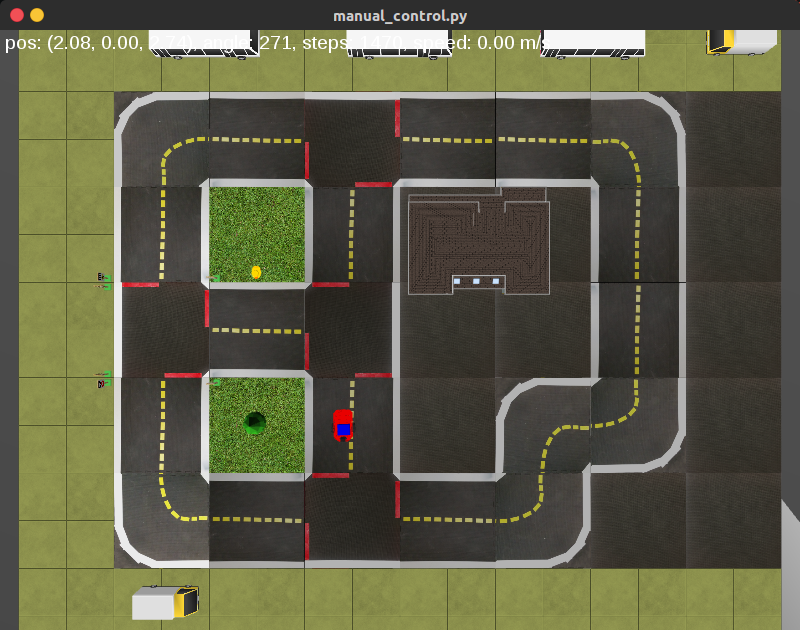
\includegraphics[width=0.6\textwidth]{kapitel2/images/duckietown-umgebung.png}
	\label{fig:duckietown-umgebung}
	\caption{Darstellung einer beispielhaften DuckieTown-Umgebung}
\end{figure}

\section{DuckieBot}

Ein \href{https://get.duckietown.com/products/duckiebot-db18}{DuckieBot} ist ein kleiner mobiler Roboter mit Differenzialantrieb, der seine Umgebung über eine Kamera wahrnehmen kann. Er ist mit einem \href{https://www.raspberrypi.org/}{Raspberry Pi} ausgestattet, welcher für Berechnungen und die Datenverarbeitung zuständig ist. Die  Räder werden über Gleichstrommotoren angetrieben. Mittels eines Steuerbefehls kann ein DuckieBot in einer Umgebung navigiert werden. \cite{duckietown_platform}

\begin{figure}[H]
	\centering
	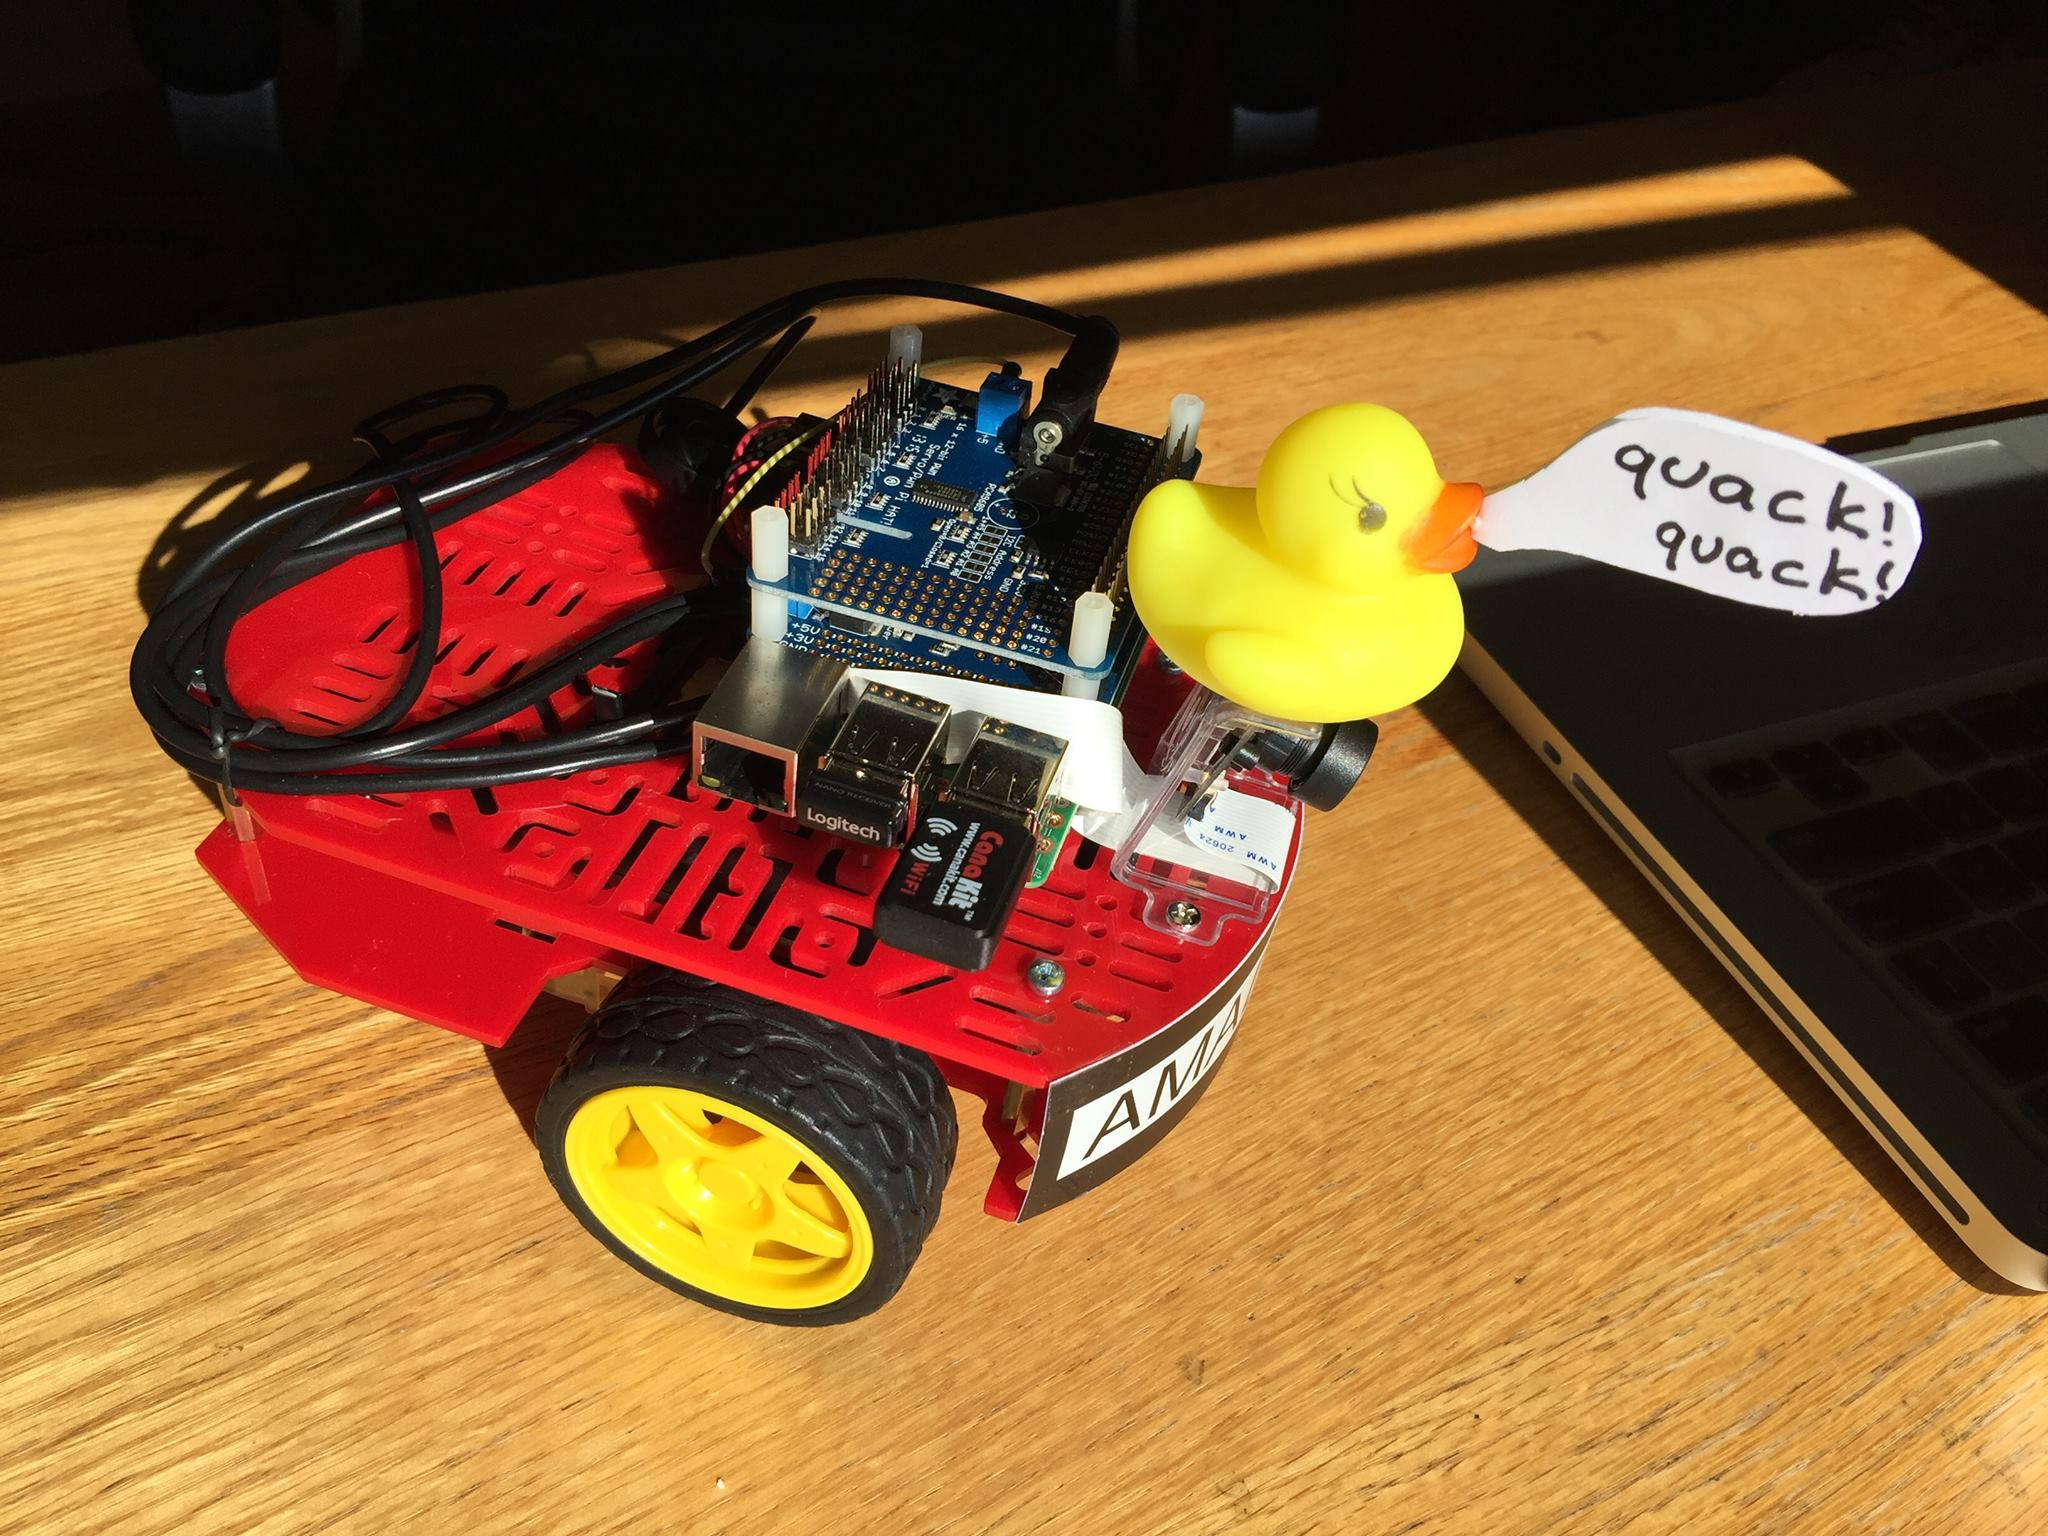
\includegraphics[width=0.5\textwidth]{kapitel2/images/duckiebot.jpg}
	\label{fig:duckiebot}
	\caption{DuckieBot}
\end{figure}


\section{Simulator}

Der \href{https://github.com/duckietown/gym-duckietown}{DuckieTown-Simulator} ist ein in \href{https://www.python.org/}{\texttt{Python}} und \href{https://www.opengl.org/}{\texttt{OpenGL}} \acf{bzw} \href{http://pyglet.org/}{\texttt{Pyglet}} geschriebener Simulator für das \glqq DuckieTown-Universum\grqq. Der Simulator bietet die Möglichkeit DuckieBots (Agenten) in einer beliebigen DuckieTown-Umgebung zu platzieren und die Agenten darin zu navigieren. Eine DuckieTown-Umgebung beinhaltet hierbei eine Menge von befahrbaren Straßenstücken, eine Menge Hindernisse, sowie nicht befahrbare Umgebungsabschnitte. \cite{gym_duckietown} \\

\begin{figure}[H]
	\centering
	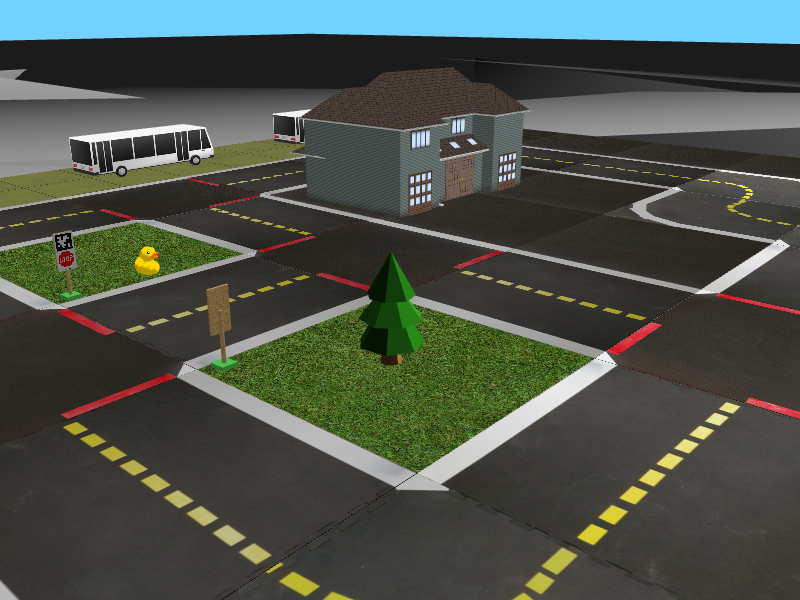
\includegraphics[width=0.6\textwidth]{kapitel2/images/duckietown-gym.png}
	\label{fig:duckietown-gym}
	\caption{DuckieTown-Simulator}
\end{figure}

Der Simulator ist schnell, quelloffen und ausgesprochen anpassungsfähig. Er wurde zunächst für die einfache Linienverfolgung konzipiert und wurde dann im Laufe der Zeit zu einem voll funktionsfähigen Simulator für autonom fahrende Fahrzeuge, insbesondere im Bezug zur künstlichen Intelligenz. \cite{gym_duckietown}

